%-----------------------------------------------------------------------------%
\chapter{\babTiga}
%-----------------------------------------------------------------------------%
Pada bagian ini akan dijelaskan metodologi yang digunakan oleh Penulis pada saat melakukan penelitian. Metodologi terdiri dari metode implementasi OpenCL dan Vulkan serta metode pengujian hasil implementasi.

\section{Metode Implementasi }
%-----------------------------------------------------------------------------%
Deep Learning Inference terdiri dari operasi-operasi matriks. Penerapan Deep Learning Inference menggunakan GPU dapat dilakukan dengan menerapkan OpenCL dan Vulkan pada operasi-operasi matriks terkait. Misalnya pada DNN inference, OpenCL dan Vulkan dapat diterapkan terhadap operasi perkalian matriks-vector untuk dijalankan pada GPU. Pada CNN inference, selain perkalian matriks juga terdapat operasi konvolusi yang dapat dijalankan melalui OpenCL dan Vulkan pada GPU. Dalam penelitian ini penulis hanya berfokus pada dua operasi, perkalian matriks dan convolution.

Implementasi Deep Learning Inference pada GPU dilakukan melalui Tensorflow Lite sebagai framework Deep Learning Inference pada perangkat mobile. Tensorflow Lite memiliki implementasi kernel berisi operasi-operasi Neural Network inference yang terpisah dari Tensorflow core. Penulis menambahkan dukungan OpenCL dan Vulkan terhadap kernel untuk operasi perkalian matriks dan konvolusi sehingga DNN dan CNN dapat dijalankan pada GPU. Tensorflow Lite tidak memiliki algoritma perkalian matrix-vector. Untuk DNN, ia menggunakan algoritma perkalian matrix biasa. Saat kompilasi, aplikasi dapat memilih untuk menggunakan default kernel (CPU), OpenCL kernel (GPU), atau Vulkan kernel (GPU). \pic~\ref{fig:modifieddiagram} menunjukkan struktur dari Tensorflow Lite dan bagian dimana OpenCL dan Vulkan diterapkan.

\begin{figure}
	\centering
	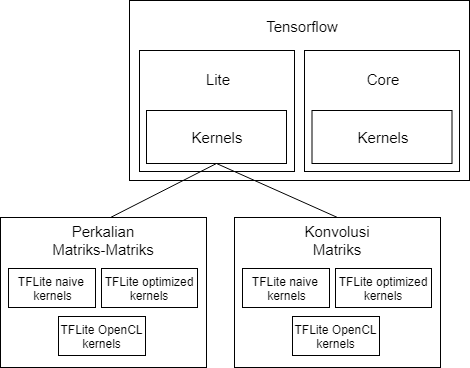
\includegraphics[width=0.50\textwidth]
	{pics/modifieddiagram.png}
	\caption{Bagian Tensorflow Lite yang dioptimasi.}
	\label{fig:modifieddiagram}
\end{figure}

Dalam mengimplementasikan perkalian matriks menggunakan OpenCL dan Vulkan, penulis menggunakan pendekatan multiplication by block (blocking). Perkalian matriks dikerjakan secara bertahap dengan membagi matriks ke dalam beberapa blok. Pendekatan ini didasarkan pada paper \cite{matmulblock}. Motivasi dari pendekatan blocking ini adalah memanfaatkan kemampuan memori lokal (dalam suatu work-group) yang lebih cepat daripada memori global. Perkalian matriks konvensional akan selalu mengambil data dari buffer yang terletak di global memory. Diketahui bahwa perkalian matriks melibatkan pembacaan data yang sama beberapa kali. Misalnya pada perkalian matriks A dan B yang menghasilkan matriks C, untuk mendapatkan nilai baris ke-i pada matriks C dilakukan dot product antara baris ke-i dari matriks A dengan setiap kolom dari matriks B. Pada perkalian matriks biasa, baris ke-i dari matriks A akan dibaca beberapa kali melalui global memory. 

Dengan melakukan perkalian matriks per-blok, keunggulan kecepatan akses local memori dapat dimanfaatkan. Pasangan blok matriks A dan B yang akan dikalikan dimuat terlebih dahulu ke local memory. Block tersebut hanya dibaca satu kali dari global memory selama proses komputasi. Ketika perkalian antar blok dilakukan, banyak data yang sama pada blok tersebut yang dibaca berkali-kali, namun kali ini dibaca melalui local memory. Dengan demikian akan lebih sedikit waktu yang terbuang untuk operasi read memory. Perhatikan bahwa setiap blok matriks masing-masing menggunakan data yang unik. Data pada blok-blok lain tidak dibaca ketika memproses suatu blok. Sehingga tidak ada data yang dibaca lebih dari satu kali dari global memory. \pic~\ref{fig:matmulblock2} menujukkan contoh perkalian matriks pada dengan blocking.

\begin{figure}
	\centering
	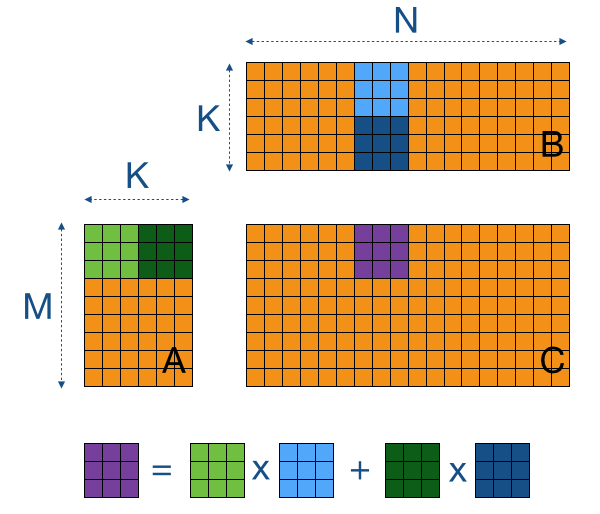
\includegraphics[width=0.50\textwidth]
	{pics/matmul-block1.png}
	\caption{Perkalian matriks per blok.}
	\label{fig:matmulblock2}
\end{figure}

Selain menggunakan block, beban komputasi dibagi ke banyak thread (work item) pada GPU. Satu thread hanya memproses perkalian untuk menghasilkan satu elemen pada matriks output. Jika matriks output merukuran MxN, maka akan terdapat MxN thread. Dengan demikian terjadi reduksi kompleksitas karena semua thread berjalan secara parallel. Kompleksitas perkalian matriks pada GPU dapat dihitung sebagai berikut.
//Hitung kompleksitas

//Pendekatan implementasi matrix convolution
Kemudian untuk mengimplementasikan konvolusi matriks juga digunakan pendekatan yang sama yaitu dengan memanfaatkan local memori untuk mempercepat proses pembacaan data. Pendekatan ini mengikuti paper \cite{convblock}. 

Implementasi perkalian matriks dan konvolusi melalui OpenCL dan Vulkan memerlukan persiapan yang cukup panjang sebelum komputasi seperti yang dijelaskan pada bagian landasan teori OpenCL dan Vulkan. Oleh karena itu, penulis mengoptimisasi proses persiapan ini dengan memindahkan beberapa persiapan ke awal mulainya aplikasi sehingga hanya dijalankan satu kali selma aplikasi berjalan. Tidak semua persiapan dapat dipindahkan ke awal jalannya aplikasi karena beberapa persiapan bergantung pada data input yang bersifat dinamis, sehingga tidak dapat dilakukan hanya satu kali ketika aplikasi dijalankan. 

// Pada OpenCL apa saja yang diawal, pada Vulkan apa saja.

\section{Metode Pengujian }
%-----------------------------------------------------------------------------%
Setelah implementasi OpenCL dan Vulkan menghasilkan keluaran yang benar, dilakukan pengujian untuk mengetahui performa dari masing-masing implementasi. Kemudian, performa dibandingkan dengan implementasi asli dari Tensorflow serta implementasi multithreading yang sudah dioptimalkan untuk arsitektur ARM. Untuk melakukan pengujian, penulis menggunakan aplikasi demo dari Tensorflow yaitu Tensorflow Lite Camera Demo yang merupakan aplikasi image recognition yang memanfaatkan CNN. Beberapa perangkat android dengan GPU Adreno dan Mali digunakan dalam pengujian ini. Selain melakukan pengujian pada perangkat android, penulis juga melakukan pengujian pada PC untuk mengetahui perbedaan performa pada PC dan android. Penulis melakukan pengujian terhadap beberapa model CNN yang mengandung convolution layer dan fully-connected layer, antara lain Inception, LeNet, dan AlexNet. 

Dalam pengujian, penulis mengamati tiga hal yaitu kecepatan inference, penggunaan memori, dan penggunaan baterai. Selain itu, penulis juga mengamati kecepatan dari masing-masing operasi perkalian matriks dan konvolusi yang terlibat saat proses inference. Penulis kemudian juga mengamati kontribusi proses-proses persiapan OpenCL dan Vulkan terhadap kecepatan dari keseluruhan inference untuk mengetahui letak bottleneck pada inference, terutama pada matriks-matriks kecil. Penulis juga membandingkan performa eksekusi kernel/shader antara OpenCL dan Vulkan untuk mengetahui performa driver dari masing-masing API.